\documentclass[msc]{ppgccufmg}

\usepackage[english]{babel}      % se o documento for em inglês
\usepackage[utf8]{inputenc}
\usepackage[T1]{fontenc}
\usepackage{type1ec}
\usepackage{graphicx}
\usepackage[a4paper,
  english,
  bookmarks=true,
  bookmarksnumbered=true,
  linktocpage,
  colorlinks,
  citecolor=black,
  urlcolor=black,
  linkcolor=black,
  filecolor=black,
  ]{hyperref}
\usepackage[square]{natbib}

\begin{document}

\ppgccufmg{
    title={A Deep Learning approach for the creation and interpretation of a Pain Scale on Fetuses},
    portuguesetitle={Criação e Interpretação de Uma Escala de Dor para Fetos Por Meio de Aprendizado Profundo},
    authorrev={Oliveira, Thiago Melo de},
    cutter={D1234p},
    cdu={519.6*82.10},
    university={Federal University of Minas Gerais},
    course={Computer Science},
    portugueseuniversity={Universidade Federal de Minas Gerais},
    portuguesecourse={Ciência da Computação},
    address={Belo Horizonte},
    date={2020-03},
    advisor={Nivio Ziviani},
    coadvisor={Adriano Veloso},
    abstract=[brazil]{Resumo}{resumo},
    abstract={Abstract}{abstract},
    dedication={dedicatoria},
    ack={agradecimentos},
    keywords={Insert Keywords Here},
    epigraphtext={Truth and lie are opposite things.}{Unknown},
    %  approval={img/approvalsheet.eps},
    %  approval=[-2.5cm][1]{aprovalsheet},
}


% Os três comandos seguintes são apenas para gerar texto para ocupar espaço nas
% páginas.
\newcommand{\dummytxta}{%
Lorem ipsum dolor sit amet, consectetur adipisicing elit, sed do
eiusmod tempor incididunt ut labore et dolore magna aliqua. Ut enim ad
minim veniam, quis nostrud exercitation ullamco laboris nisi ut
aliquip ex ea commodo consequat. Duis aute irure dolor in
reprehenderit in voluptate velit esse cillum dolore eu fugiat nulla
pariatur. Excepteur sint occaecat cupidatat non proident, sunt in
culpa qui officia deserunt mollit anim id est laborum.\par
}

\newcommand{\dummytxtb}{%
Sed ut perspiciatis unde omnis iste natus error sit voluptatem accusantium
doloremque laudantium, totam rem aperiam, eaque ipsa quae ab illo inventore
veritatis et quasi architecto beatae vitae dicta sunt explicabo. Nemo enim
ipsam voluptatem quia voluptas sit aspernatur aut odit aut fugit, sed quia
consequuntur magni dolores eos qui ratione voluptatem sequi nesciunt. Neque
porro quisquam est, qui dolorem ipsum quia dolor sit amet, consectetur,
adipisci velit, sed quia non numquam eius modi tempora incidunt ut labore et
dolore magnam aliquam quaerat voluptatem. Ut enim ad minima veniam, quis
nostrum exercitationem ullam corporis suscipit laboriosam, nisi ut aliquid ex
ea commodi consequatur? Quis autem vel eum iure reprehenderit qui in ea
voluptate velit esse quam nihil molestiae consequatur, vel illum qui dolorem
eum fugiat quo voluptas nulla pariatur?\par
}

\newcommand{\dummytxtc}{%
At vero eos et accusamus et iusto odio dignissimos ducimus qui blanditiis
praesentium voluptatum deleniti atque corrupti quos dolores et quas molestias
excepturi sint occaecati cupiditate non provident, similique sunt in culpa qui
officia deserunt mollitia animi, id est laborum et dolorum fuga. Et harum
quidem rerum facilis est et expedita distinctio. Nam libero tempore, cum soluta
nobis est eligendi optio cumque nihil impedit quo minus id quod maxime placeat
facere possimus, omnis voluptas assumenda est, omnis dolor
repellendus. Temporibus autem quibusdam et aut officiis debitis aut rerum
necessitatibus saepe eveniet ut et voluptates repudiandae sint et molestiae non
recusandae. Itaque earum rerum hic tenetur a sapiente delectus, ut aut
reiciendis voluptatibus maiores alias consequatur aut perferendis doloribus
asperiores repellat.\par
}

\newcommand{\dummytxt}{\dummytxta\dummytxtb\dummytxtc}

\chapter{Introdução}

Segundo \cite{horn86robot}, todo triângulo equilátero tem os lados iguais. Já
segundo \cite{shashua97photometric}, todo quadrado também tem.

Veja que o pacote \verb|natbib| permite uma série de formas diferentes para
fazer referências bibliográficas. O comando padrão, \verb|\cite|, realiza a
citação comum vista no parágrafo anterior. Outros comandos permitem, por
exemplo, citar somente o autor --- por exemplo, citar o trabalho de
\citeauthor{samaras99coupled} --- ou colocar automaticamente a citação entre
parênteses \citep{hougen93estimation, sato99illumination2, sato99illumination1,
sato01stability}. Os comandos usados foram, respectivamente, \verb|\citeauthor|
e \verb|\citep|. Veja a documentação do \verb|natbib| na Internet para conhecer
outros comandos e exemplos de uso.

Citações aleatórias para fazer com que as referências bibliográficas ocupem
mais de uma página: \cite{bichsel92simple, dror01statistics, guisser92new}.


\section{Motivação}

\dummytxtb\dummytxta

\subsection{Sub-motivação}


\dummytxtc\dummytxtb

\subsection{Mais uma sub-seção}

\dummytxta\dummytxtc

\subsubsection{Descendo mais um nível}

\dummytxtb\dummytxta


\chapter{Desenvolvimento}

\dummytxtb\dummytxta\dummytxtc

\begin{figure}[t]
    \centering
    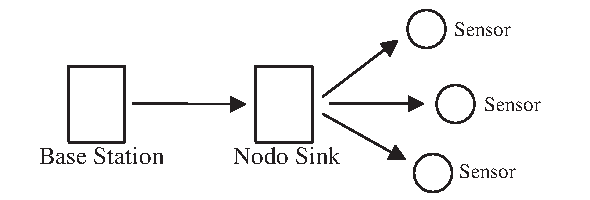
\includegraphics{img/exemplo}
    \caption{Uma figura de exemplo.}
    \label{fig:exemplo}
\end{figure}

\dummytxtb\dummytxta\dummytxtc\dummytxtb

\begin{table}[t]
    \caption{Uma tabela de exemplo.}
    {\centering
    \begin{tabular}{lcr} \toprule
    \emph{Left-aligned} & \emph{Centered} & \emph{Right-aligned} \\ \midrule
    Lorem ipsum & dolor sit & amet \\
    consectetur adipisicing & elit, sed do eiusmod & tempor \\
    incididunt ut & labore et dolore & magna aliqua. \\ \bottomrule
    \end{tabular}\par
    }
\end{table}


% Aqui vem a parte da bibliografia: use o comando \ppgccbibliography indicando
% apenas o nome do arquivo .bib (sem a extensão).
\ppgccbibliography{bibfile}


% Este comando encapsula o conjunto de apêndices. A sua função é fazer com que
% a numeração dos apêndices seja feita com letras maiúsculas (A, B, C, etc.) e
% a palavra "Apêndice" anteceda as entradas no Sumário.
\begin{appendices}

% Para cada apêndice, um \chapter
\chapter{Um apêndice}

\dummytxta
\dummytxtb
\dummytxtc
\dummytxta
\dummytxtb

\chapter{Outro apêndice}

\dummytxta
\dummytxtb
\dummytxtc
\dummytxta
\dummytxtb

% Fim dos apêndices (usar apenas depois do último apêndice)
\end{appendices}


% Este comando encapsula o conjunto de anexos. A sua função é fazer com que a
% numeração dos anexos seja feita com letras maiúsculas (A, B, C, etc.) e a
% palavra "Anexo" anteceda as entradas no Sumário.
\begin{attachments}

% Para cada anexo, um \chapter
\chapter{Um anexo}

\dummytxta
\dummytxtb
\dummytxtc
\dummytxta
\dummytxtb

\chapter{Outro anexo}

\dummytxta
\dummytxtb

% Fim dos anexos (usar apenas depois do último anexo)
\end{attachments}


\end{document}
